%-------------------------------------------------------------------------------
% patterns_panel
%-------------------------------------------------------------------------------
%
% \file        patterns_panel.tex
% \library     Documents
% \author      Chris Ahlstrom
% \date        2015-08-31
% \update      2022-02-12
% \version     $Revision$
% \license     $XPC_GPL_LICENSE$
%
%     Provides the concepts.
%
%-------------------------------------------------------------------------------

\section{Patterns Panel}
\label{sec:patterns_panel}

   \textsl{Seq66} works with patterns (also known as "loops", "tracks", or
   "sequences") that are repeated throughout a song.
   One composes and edits small patterns in a grid,
   and combines them to create a full song.
   This is a powerful way to work, and makes one productive quickly.

   \index{Patterns Panel}
   \index{Live Frame}
   \index{Live Grid}
   The \textbf{Patterns Panel}, also called the
   \textbf{Live Frame} or
   \textbf{Live Grid} or
   is in the center of the
   \index{main window}
   \textbf{main window} of \textsl{Seq66}.
   See \figureref{fig:main_screen}.
   It is here one creates a set of patterns ("screenset"),
%  (see \sectionref{subsubsec:concepts_terms_screen_set}),
   manages the configuration, controls the playback rate, adds tempo events,
   and opens the pattern, song, event, mute-groups, or playlist editors.

%  \index{live mode}
%  \index{mode!live}
%  \index{mode!song}
%  When the patterns panel has the focus,
%  and \textsl{Seq66} is \textsl{not} running in \textbf{Song} mode,
%  it puts \textsl{Seq66} in \textbf{Live} mode.
   The musician can
   control the playback and muting/unmuting of each pattern in
   the song, while it is playing, from within this window.
   One can also switch to other screensets, to work with a different
   part of the song.

%  \index{song mode}
%  \index{mode!song}
%  If the song editor (see \sectionref{sec:song_editor})
%  has the input focus, it automatically controls the muting/unmuting of
%  each pattern, and \textsl{Seq66} runs in \textbf{Song} mode.
%  (There are ways to override this behavior, such as the
%  \textbf{Song/Live} button.)

   For exposition, we divide the patterns panel
   into a menu bar, a top panel, a pattern panel (live frame/grid),
   and a bottom panel.
   The \textsl{Seq66} menu bar is discussed in \sectionref{sec:menu}.

\subsection{Patterns / Main Panel}
\label{subsec:patterns_panel_main}

   The main panel of the application provides a grid of empty boxes,
   as shown in
   \figureref{fig:patterns_panel_popup_menu}.
   Each filled box represents a loop, track, sequence, or pattern
   (interchangeable terms).
   One sees only 32 loops at a time in the main panel (but many more than
   32 loops can be supported by \textsl{Seq66}).

   \index{screen-set}
   This group of 32 loops is called a "screen-set".
   One can switch between sets by using the
   \index{keys![}
   \index{keys!screenset down}
   "\texttt{[}" and
   \index{keys!]}
   \index{keys!screenset up}
   "\texttt{]}" keys on the keyboard, or by using
   the spin-widget-driven, labelled \textbf{Set} interface item, or
   \index{keys!Home}
   \index{keys!screenset play}
   by hitting the (default) \texttt{Home} key to make it the playing screenset,
   or by hitting \texttt{Page-Up} or \texttt{Page-Down} with the pattern window
   in keyboard focus.
   There are a total of 32 sets, for a total of 1024 loops/patterns. 
   Only one screen-set can be controlled at a time, in general.
%  have found; have not yet tried to verify this assertion.
   Multiple screensets can be playing at the same time, depending on
   configuration.

   The \texttt{Page Up} and \texttt{Page Down}, and \texttt{Up/Down Arrow}
   keystrokes can be used inside of the \textbf{Set} spin-button.

   It is important to note that, currently, incrementing or decrementing
   the screen-set will \textsl{not} wrap-around.
   We consider this a feature rather than a bug, at this time.

   There are some other important considerations for set-handling.
   See \sectionref{sec:setmaster}.

\begin{figure}[H]
   \centering 
   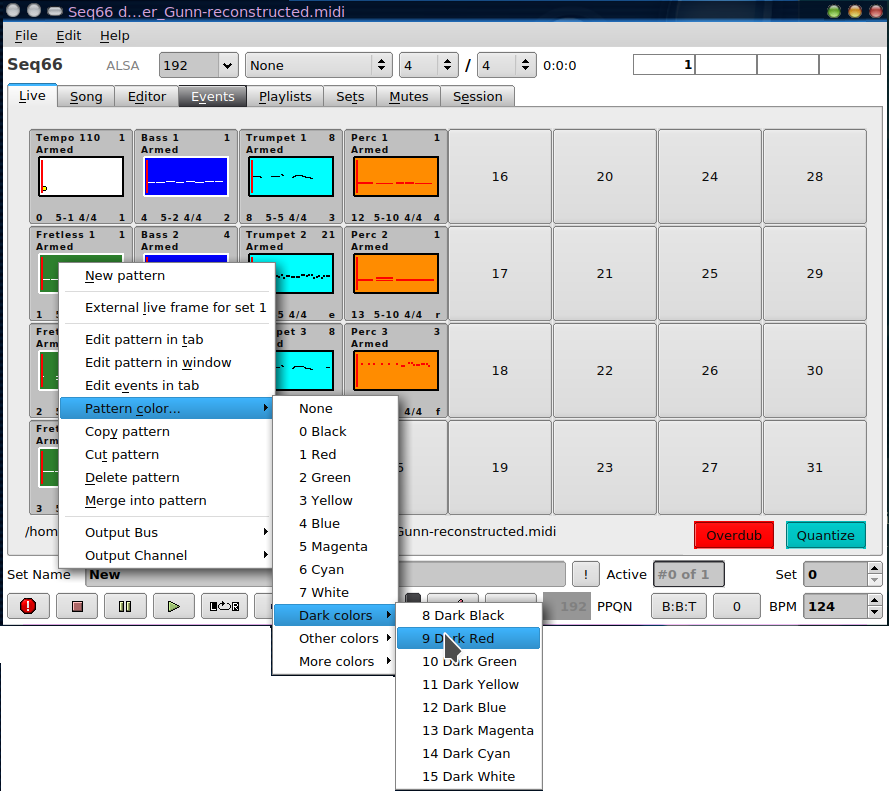
\includegraphics[scale=0.75]{tabs/live/pattern-popup-menu.png}
   \caption{Patterns Panel Pop-up Menu}
   \label{fig:patterns_panel_popup_menu}
\end{figure}

   The individual items annoted in this figure are described in
   \sectionref{subsubsec:patterns_pattern_filled}, in more detail.

   Also note buttons for changing and showing the
   loop/recording modes of the grid buttons and recording quantization.
   \textsl{Seq66}'s pattern grid can be put in various recording
   modes (e.g. overdub/merge versus overwrite) where, instead of
   muting/unmuting the patterns, it turns on recording (without opening the
   pattern editor).
   Quantization can be turned on globally in \textsl{Seq66}'s pattern grid
   as well.
   These operations are also available as automation controls.
   See \sectionref{paragraph:configuration_midi_record_quan}.

   Observe that feature in the first figure of the next section.
   The two main items are the empty \textsl{pattern slot}, and the slot filled
   with a MIDI \textsl{pattern}:

   \begin{enumber}
      \item \textbf{Pattern Slot}
      \item \textbf{Pattern}
   \end{enumber}

\subsubsection{Pattern Slot}
\label{subsubsec:patterns_pattern_slot}

   \index{pattern!slot}
   An empty box is a slot for a pattern.
   If a pattern is present in the slot, text information and notes are drawn on
   the button.
   For example, the top line will show
   the title of the pattern, the number of measures in the pattern, and
   indicate if the pattern has a loop-count.
   A right-click over a pattern button brings up a fairly extensive
   popup menu.
   Also see \sectionref{subsubsec:patterns_pattern_filled}.

%  The slot at the bottom left of this figure shows the features:
%
%  \begin{itemize}
%     \item The sequence number (from 0 on up) appears at the bottom left of
%        the slot.
%     \item The buss number (re 0) and the channel number (re 1) appears
%        to the right of the sequence number, in the format "0-1".
%     \item To the right of that, the time signature ("4/4") appears, at the
%        bottom.
%     \item The hot-key for muting/unmuting the pattern appears next,
%        at the bottom right of the slot.
%     \item The title of the sequence appears at the top left of the pattern
%        slot.
%     \item The length of the sequence, in number of measures (bars), appears
%        at the upper right of the slot.
%     \item The font is a \textsl{Qt} font.
%  \end{itemize}

   A pattern can show a number of different statuses based on the coloring
   of elements in the pattern slot.
   (However, note that some of the special coloring using in
   \textsl{Sequencer64} is not supported in \textsl{Seq66}.

   \begin{itemize}
      \item \textbf{Empty background}.
         When the default button coloring for
         the current \textsl{Qt} theme is shown, without a pattern box,
         this state indicates that the slot is unused.
      \item \textbf{Yellow pattern box}.
         This color is used when a pattern is
         first created by double-clicking on the slot.
         However, this color sticks even when notes are added.
         Feel free to change it to another color, or no color.
      \item \textbf{Normal background}.
         Unarmed (muted) patterns show the
         unactivated/unchecked state of the button as per the \textsl{Qt}
         theme.  If a color is applied, it has a slight bit of alpha in the
         color so that the color appears muted.
      \item \textbf{Active background}.
         An armed (unmuted) pattern shows the
         activated/checked state of the button as per the \textsl{Qt}
         theme.  If a color is applied, it has no transparency, and the 
         color appears bright.
      \item \textbf{Line events}.
         \index{event!note}
         Lines indicate the presence of notes.  Depending on settings, the
         lines indicate the notes themselves, or a "fingerprint", a condensed
         indication of notes useful in reducing the overhead of
         drawing long patterns.
      \item \textbf{Red events}.
         \index{event!drum note}
         Indicates a pattern for which the transpose feature is
         disabled.  Most useful with drum patterns.
      \item \textbf{Circular events}.
         \index{event!tempo}
         Small circles indicate tempo events.  Generally, these events should
         appear only in the tempo track (which is normally track 0).
   \end{itemize}

   The user can also apply coloring to each sequence.
   This feature was adopted from \textsl{Kepler34} \cite{kepler34}.
   The color is more saturated when the pattern is unmuted.
   \index{pattern!color menu}

   \index{pattern!right click}
   \index{slot!empty slot right-click}
   Right-clicking on an empty box one brings up a menu to create
   a new loop or open an external live grid, as well as some other operations.

   \begin{enumber}
      \item \textbf{New pattern}
      \item \textbf{External live frame for set 0}
   \end{enumber}

   \setcounter{ItemCounter}{0}      % Reset the ItemCounter for this list.

   \itempar{New}{pattern!new}
   Creates a new loop or pattern.
   Clicking this menu entry fills in the empty box with an untitled
   pattern.  Another way to create a new loop is to double-left-click on an
   empty slot; this also brings up an external pattern editor (discussed
   later).

   \itempar{External live frame for set 0}{live!external}
   This option brings up an external \textbf{Live} frame window, which
   is the same as the patterns panel, but can be used to show a different set
   in a multi-set project.  Up to 32 external live frames can be shown.
   An external live grid can be activated by the \textbf{Activate} button,
   which sets the playing screen-set
   (and updates the main window to match).

\begin{figure}[H]
   \centering 
   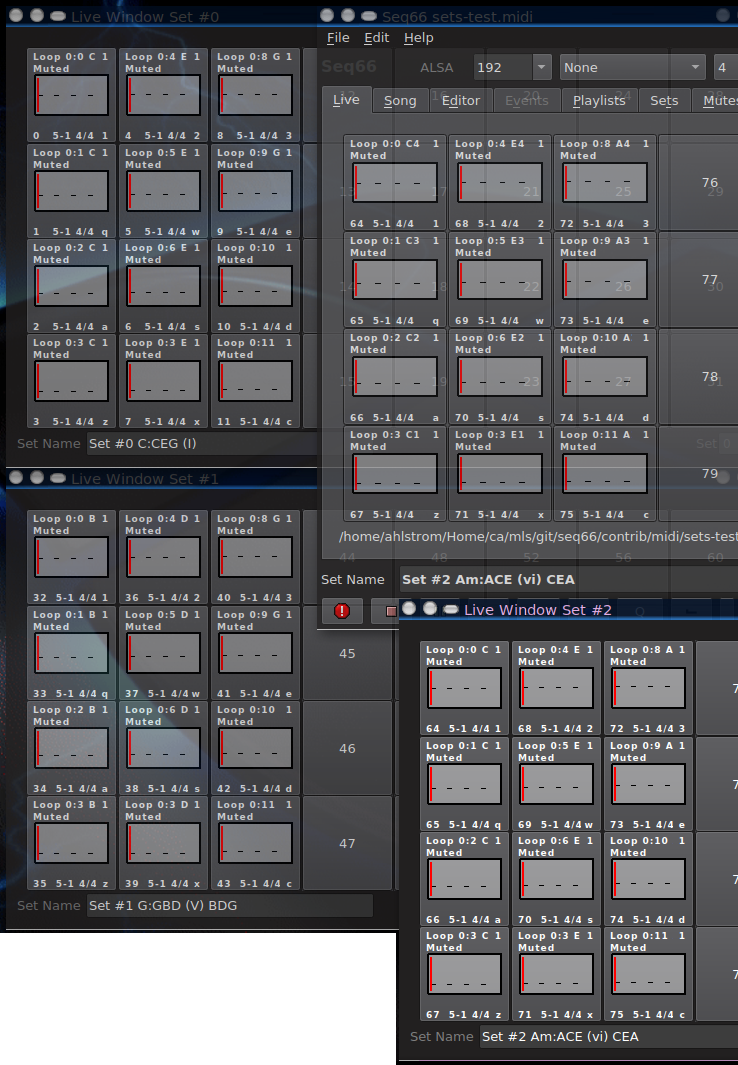
\includegraphics[scale=0.65]{main-window/multiple-live-grids.png}
   \caption{Multiple Live Grids}
   \label{fig:multiple_live_grids}
\end{figure}

   Note that the right-click slot menu has some items removed when the live
   grid is in an external window, or the main window is showing a set other
   than set 0 , as indicated by
   the asterisks in the list below.
   We hope to rectify that in a future release.

   Once a new loop is created, there are more options for that slot.
   \index{pattern!right click}
   A right-click on an already-filled box brings up a menu
   to allow one to edit it, or perform a few other actions
   specified in the context menu.  Here is that menu:

   \begin{enumber}
      \item \textbf{New pattern}
      \item \textbf{External live frame for set ...} *
      \item \textbf{Edit pattern in tab} *
      \item \textbf{Edit pattern in window} *
      \item \textbf{Edit events in tab} *
      \item \textbf{Set pattern color}
      \item \textbf{Copy pattern}
      \item \textbf{Cut pattern}
      \item \textbf{Delete pattern}
      \item \textbf{Merge into pattern}
      \item \textbf{Output Bus}
      \item \textbf{Output Channel}
   \end{enumber}

   The first menu entry is the same as above.  However, since there is
   already a pattern present in the slot, the user is prompted before erasing
   the current pattern and creating a new one.

   \setcounter{ItemCounter}{0}      % Reset the ItemCounter for this list.

   \itempar{New Pattern}{pattern!new}
   Creates a new pattern in the empty slot.
   \index{slot!double-click}
   Can also be done by double-clicking on an empty slot.

   \itempar{External Live Frame for Set}{pattern!external live frame}
   This selection uses the pattern number to open the corresponding screenset
   number in an external \textbf{Live} frame.
   This allows viewing and interacting with a number of sets.

   \itempar{Edit Pattern In Tab}{pattern!edit in tab}
   Selecting this item activates the \textbf{Edit} tab and fills it with data
   from the selected pattern.
   Note that this editor is somewhat simplistic, useful for trouble-shooting a
   pattern.

   \itempar{Edit Pattern In Window}{pattern!edit in window}
   Selecting this item brings up the pattern in an external pattern editor that
   has a few addition controls over the \textbf{Edit} tab (where space is more
   constrained).

   In addition to right-click and select \textbf{New}, the user can
   \index{empty slot double-click}
   double-click on the empty slot, to bring up a new instance of the sequence
   editor.  For double-click on an existing pattern,
   the effect can be a bit confusing at first,
   because it also toggles the armed/muted status of the slot
   quickly twice (leaving it as it was).

   \index{editing shortcut}
   \index{keys!=}
   \index{keys!pattern edit}

   A nice feature is hitting the equals ("=") key, then hitting
   a pattern shortcut key (hot-key), to bring up a new sequence or edit an
   existing one in a \textbf{Pattern Editor} .

   \itempar{Edit Events In Tab}{pattern!events in tab}
   Edits an existing loop or pattern, but using a detailed \textbf{Event Editor}
   tab that shows events as text and numbers, and allows editing them as text
   and numbers.
   This editor is basic, meant for viewing
   MIDI events and making some minor edits or deletes.
   The \textbf{Event Editor} is most useful when trying to find events
   that are screwing up the performance of that pattern.
   See \sectionref{sec:event_editor}, for more information.

   \index{keys!-}
   \index{keys!event edit}
   Another feature is hitting the minus
   ("-") key, then the hot-key, to bring up the \textbf{Event Editor} tab.
   The configuration file settings for the the '=' and
   '-' keys can be altered in the 'ctrl' file.

   \itempar{Set Pattern Color}{pattern!color}
   Opens a menu to select a color for the pattern.  This selects a color
   palette value (index) into the currently loaded color palette.
   See \sectionref{sec:palettes}.

   \itempar{Copy Pattern}{pattern!copy}
   Copies the pattern underneath the mouse cursor.
   The pattern can then be pasted elsewhere in the Patterns panel.
   One can also drag-and-drop a pattern into another cell (there is no outline
   box during the drag, unfortunately).
   See \sectionref{subsubsec:patterns_pattern_slot}.
   Note that there is no \texttt{Ctrl-C} key for this operation in the
   live (main) window.

   \itempar{Cut Pattern}{pattern!cut}
   Cuts the pattern while copying it for later pasting.
   There is no \texttt{Ctrl-X} key for this operation.

   \itempar{Delete Pattern}{pattern!delete}
   Deletes the pattern.  Currently the same as Cut!

   \itempar{Paste Pattern}{pattern!paste}
   Pastes a loop or pattern that was previously copied.
   This option is shown only when right-clicking over an empty pattern.
   It causes a cut or copied pattern to be replicated into the emptly slot.
   Note that there is no \texttt{Ctrl-V} key for this operation in the
   main window.

   \itempar{Merge Into Pattern}{pattern!merge}
   This item is a new feature.  Like \textbf{Paste to pattern}, it pastes a
   patten that was cut or copied into the pattern slot where the mouse was
   right-clicked.  However, the original notes remain.  Thus, the merge
   option provides a way to build up a pattern by copying other patterns.

   \itempar{Output Bus}{pattern!buss}
   This item allows one to select the output buss for a pattern without having
   to open the editor.

   \itempar{Output Channel}{pattern!channel}
   This item allows one to select the output channel for a pattern without
   having to open the editor.
   
\subsubsection{Pattern}
\label{subsubsec:patterns_pattern_filled}

   A filled pattern slot is referred to as a \textsl{pattern}
   (or \textsl{track}, \textsl{loop}, or \textsl{sequence}).
   A pattern is shown in the pattern grid as a filled box with a number of
   items of information surrounding it.  Here are the items shown:

   \begin{itemize}
      \item \textbf{Pattern Name}. Top left.
         \index{pattern!name}
         This line, in the upper left of the pattern slot, contains the name or
         title of the pattern, for reference when juggling a number of
         patterns.
      \item \textbf{Pattern Status}. Second line.
         \index{pattern!status}
         Underneath the pattern-name is the status of the pattern, such as
         "Armed", "Muted", or "Queued".
         This status is useful when the Qt theme coloring makes the exact
         status difficult to determine.
      \item \textbf{Pattern Length}. Top right.
         \index{pattern!length}
         The length of the pattern, in measures, is shown in the upper
         right corner of the pattern slot.
         Also, if the loop-count for the pattern is greater than 0, 
         then an \textbf{asterisk} is shown.
         Remember that a pattern loop-count of 0 means the pattern can repeat
         "forever".
      \item \textbf{Notes or Fingerprint}. Center.
         \index{pattern!contents}
         The contents of the pattern, in the central box,
         provide a distinguishable representation of the notes or events in the
         pattern.
         The notes are shown in the center, inside a "progress box" that
         can also be colored, or not shown at all.
         Long patterns can be replaced by a much shorter "fingerprint", for
         faster drawing.
         Tempo events are indicated by a small circle.
         \index{empty pattern}
         An pattern with no playable events will not needlessly scroll.
         However, if a pattern has even a single event (say, a program change),
         it will scroll.
      \item \textbf{Progress Cursor}. Center.
         At the left of each center box is a vertical line, waiting for
         playback to start so that it can move through the pattern, again and
         again.
         When the song is playing, this vertical bar
         tracks the position of the playback of the pattern or loop; it
         returns to the beginning of the box every time the pattern starts
         over.
%        \index{todo:one-shot pattern}
%        It might be good to have some patterns marked as one-shot patterns.
%        They play once at the start of playback, and that is it.
%        They could be marked with a cyan background.
%        Currently, it is easy enough to use the Song Editor for this purpose,
%        but then one cannot play the patterns in live mode.
      \item \textbf{Sequence Number}. Bottom left.
         This number is shown at the bottom left of the pattern slot.
         Pattern numbers, by default, range from 0 to 31.
         Note how it varies fastest by row (top to bottom).
      \item \textbf{Bus-Channel}. Bottom, second from left.
         \index{pattern!bus-channel}
         This pair of numbers shows the the MIDI buss number, a dash, and
         the MIDI output channel number.
         For example, "0-2" means MIDI buss 0 (re 0), channel 2 (re 1).
         \index{pattern!free channel}
         If the channel is an "F", this means that the pattern has no specified
         output channel, and can play on all channels.
         This "free" channel concept is useful for applying Program Changes and
         Volume controls to many channels at once.
      \item \textbf{Beat/Beat Width}. Bottom, third from left.
         \index{pattern!beat}
         This pair of numbers is the standard time-signature of the pattern,
         such as "4/4" or "3/4".  The first number is the beats-per-measure,
         and the second is the size of the beat, here, a quarter note.
      \item \textbf{Shortcut Key}.  Bottom right.
         The key noted in the lower-right corner of the pattern is a "hot-key"
         that can be pressed to toggle the mute/unmute status of that pattern.
         This action is an alternative to left-click on the pattern.
         This hot-key can also be used to open the pattern in a pattern editor
         or in the event editor.
      \item \textbf{Armed}. Highlight color of button.
         Button highlighting indicates that the pattern is armed
         (unmuted), and will play if playback is initiated in the pattern
         \index{live mode}
         window in live mode.
         An item is armed/disarmed by a left-click on it, or by using the
         button's hot-key.
      \item \textbf{External Frame}. Shift-left-click.
         \index{shift left click}
         If the \texttt{Shift} key is held during a left-click on a pattern,
         the corresponding set's \textbf{Live} frame is brought up.
   \end{itemize}

   \index{pattern!left click}
   Left-click on an filled pattern box will toggle the status of the
   pattern between muted (white background) and unmuted (black background).
   If the song is playing via the main window, toggling this status makes
   the pattern stop playing or start playing.  The armed status
   can also be toggled using hot-keys and MIDI controls.

%  \itempar{Cut}{pattern!cut}
%  Deletes and copies an existing loop or pattern.

% =========================================================================

%  \itempar{MIDI Bus}{pattern!midi bus}
%  Selecting this filled-box right-click menu item brings up a list
%  of the up to 16 MIDI output busses that \textsl{Seq66} supports.
%  For each of these buss items, another pop-up menu allows one
%  to specify the MIDI output channel for that buss.

\subsubsection{Pattern Keys and Click}
\label{subsubsec:patterns_pattern_keys_and_clicks}

   This section recapitulates all the clicks and keys that perform actions
   in the Pattern windows.  Some additional clicks and keys are noted here
   as well.

\paragraph{Pattern Keys}
\label{paragraph:patterns_pattern_keys}

   \index{keys!hot}
   \index{keys!shortcut}
   Each pattern in the patterns panel can have a hot-key or shortcut-key
   associated with it.

   \index{keys!pattern toggle}
   \textbf{Pattern Toggle}.
   Like a left-click, for each pattern, its assigned hot-key will
   also toggle its status between muted/unmuted (armed/unarmed).
   Here is the normal layout of patterns, which was built into
   \textsl{Seq24}'s "DNA":

   \begin{verbatim}
      [  0 ] [  4 ] [  8 ] [ 12 ] [ 16 ] [ 20 ] [ 24 ] [ 28 ]
      [  1 ] [  5 ] [  9 ] [ 13 ] [ 17 ] [ 21 ] [ 25 ] [ 29 ]
      [  2 ] [  6 ] [ 10 ] [ 14 ] [ 18 ] [ 22 ] [ 26 ] [ 30 ]
      [  3 ] [  7 ] [ 11 ] [ 15 ] [ 19 ] [ 23 ] [ 27 ] [ 31 ]
   \end{verbatim}

   There is an alternate (and fairly new) mapping that can be enabled
   using the \texttt{swap-coordinates} option in the 'usr' file.
   See \sectionref{subsubsec:usr_file_user_interface_settings}.

   Below is the default keyboard "grid" that is
   mapped to the loops/patterns on the screen-set.

   \begin{verbatim}
      [ 1 ][ 2 ][ 3 ][ 4 ][ 5 ][ 6 ][ 7 ][ 8 ]
      [ q ][ w ][ e ][ r ][ t ][ y ][ u ][ i ]
      [ a ][ s ][ d ][ f ][ g ][ h ][ j ][ k ]
      [ z ][ x ][ c ][ v ][ b ][ n ][ m ][ , ]
   \end{verbatim}

   These characters are shown in the lower right corner of each
   pattern, as an aid to memory.
   This grid can be changed in the 'ctrl' file in the
   \texttt{[loop-control]} section.
   However, it is best to leave this setup as is, except for the key-swapping
   needed for alternative keyboard layouts like "QWERTZ".

   \index{keys!pattern shift}
   \textbf{Pattern Shift}.
   A "shift" functionality is available for the
   mute/unmute hot-keys when a set is larger than 32 patterns.
   \index{keys!slash}
   \index{variset!slash key}
   Normally, pressing the \texttt{1} key will toggle
   sequence 0.  If preceded by one slash key (\texttt{/}), then sequence 32
   will be toggled.  If preceded by two slash keys, then sequence 64 will be
   toggled.  This features supports using set sizes of 32, 64, and 96 patterns.

   \index{keys![}
   \index{keys!decrement set}
   \index{keys!screenset down}
   \textbf{Screenset Increment and Decrement}.
   The "\texttt{[}" and
   \index{keys!]}
   \index{keys!increment set}
   \index{keys!screenset up}
   "\texttt{]}" keys on the keyboard decrement or increment the set number.

   \index{keys!alt}
   \index{keys!snapshot}
   \textbf{Snapshot}.
   When a snapshot key is pressed, the state of the patterns
   (armed versus unarmed) is saved.  While the
   snapshot is in force, one can then change the state of the patterns
   (using the keyboard or MIDI controls, \textsl{not} the mouse)
   to change how the song plays.  When the snapshot mode is exited, the
   original saved state of the patterns is restored.

   Unlike in \textsl{Seq24}, the \texttt{Alt} keys are not used.
   In addition, the snapshot key acts like a toggle... no need to hold it down.
   Lastly, there is only one snapshot key slot.
   Our preference is to use something that does not trigger desktop
   commands, perhaps "\texttt{F11}" or "\texttt{F12}", or one of the keys in
   the keypad.
   Configured in the 'ctrl' file
   \texttt{[automation-control]} section.

   \index{keys!right ctrl}
   \index{keys!queue}
   \index{queue!temporary}
   Pressing the "queue" key and then hitting a pattern hot-key
   will queue an on/off toggle for a pattern when the end of the loop is
   reached.
   This is the "queue" functionality.
   This means that the change in state of the pattern will not take hold
   immediately, but will kick in when the pattern restarts.
   This pending state is indicated by coloring the central box of the
   pattern grey.
%  Once queing finishes, the queue mode is automatically exited.
   Please note the "keep queue" functionality and
   the "one-shot queue" functionality described below.

   A light-grey color is used to show a "one-shot" queue.
   The one-shot queue can only turn a pattern on, and it
   will force the pattern off after one play.
   Queue also works for mute/unmute pattern sets ("groups"); in this case,
   every sequence will toggle its status after its individual loop ends. 

   \index{keys!avoid ctrl/alt}
   We do \textbf{not}
   recommend using \texttt{Ctrl} or \texttt{Alt}
   keys for pattern control.  They conflict with application or desktop
   settings.
%  However, if one insists on such hot-key combinations,
%  use the \textbf{Menu} button in the main
%  window to disable the menu.
%  One can also use normal keys to enable queuing.
%  For example, the minus key or the keypad's slash key can be used.

   \index{keys!keep queue}
   \index{queue!keep}
   Pressing the "keep queue" hot-key
   \index{rc file}
   assigned in the 'rc' file activates a "sticky" queue mode.
   In this mode, pressing a pattern key immediately turns on queuing, instead
   of mute/unmute.  And multiple patterns can be handled in this way at the
   same time.
   Keep-queue persists until one clicks the queue hot-key again,
   or changes the active (viewed) screen-set. 
%  After pressing the "keep queue" hot-key, individual pattern
%  toggles are queued rather than happening immediately.
%  While in queue mode, pressing a patterns hot-key, or clicking on the
%  pattern, queues that pattern to change state at the beginning of the next
%  loop.
   \index{queue!cancel}
   “Keep queue” mode is cancelled by pressing the normal queue hot-key.
   There is also a \textbf{Q} button for the same purpose.
   Also note the "queued replace/solo" functionality, described a bit later.

   \index{one-shot queue}
   \index{keys!one-shot queue}
   \index{queue!one-shot}
   Thanks to \textsl{Kepler34}, we have "one-shot queue"
   functionality.  This one-shot setup queues a pattern up for unmuting only,
   and, once the pattern has played, it is automatically muted.  This process
   is easier than having to unqueue the pattern manually before the next
   playback.
   This hot-key can be changed in the
   \textbf{File / Options / Ext Keys / One-shot queue} field.

   \index{keys!replace}
   The "replace" hot-key sets a form of muting/unmuting.
   When the "replace" hot-key is
   pressed, then pressing a pattern's hot-key,
   that sequence is unmuted, and all of the other sequences are muted.

%  Again, \texttt{Ctrl}
%  is a very inconvenient default, so an alternative key mapping
%  should be set up in the 'rc' file via the \textbf{File / Options / Keyboard}
%  tab.
   "Replace" is a form of "solo".
   "Replace" is also implemented via MIDI control,
   where the MIDI control can be activated, but then the user has to select
   the desired sequence.  

   \index{queue!replace}
   \index{queue!solo}
   \textsl{Seq66} provides an extension to the replace/solo functionality
   that is called "queued-replace" or "queued-solo".  In this feature, when
   the "keep queue" function is activated, the replace function is queued so
   that it does not occur until the next time the patterns loop.
   And queued-replace provides a form of snapshot, limited to the
   \textsl{current} screen-set.
   Here are the steps:

   \begin{enumber}
      \item Start playback with some patterns on. 
      \item Press and release
         the "keep queue" hot-key.  This puts the application into "queue" mode.
         It is indicated via a "\textbf{Q}" button.
      \item Press and hold the "replace" hot-key.
      \item Click the desired pattern hot-key.  Observe that it arms or
         stays on, and that the other playing patterns show the "queued" color
         (grey).  At the end of the loop, they turn off, and the "replace"
         pattern is now solo.
      \item Click the same pattern hot-key again.  Observe that the other
         patterns that were toggled off are now queued to be toggled on at the
         next loop.  Steps 4 and 5 can be repeated endlessly.
      \item To end
         \index{queue!clear}
         \index{queue!end}
         the "queued-replace" mode, click the normal "queue"
         hot-key.  Also, changing the active screen-set ends "queue-replace"
         mode.  It does \textsl{not} end normal queue mode, to preserve the
         behavior found in \textsl{Seq24}.
         One needs to clear the queue mode in order to select another pattern
         to solo.
   \end{enumber}

% \begin{figure}[H]
%  \centering 
%  \includegraphics[scale=0.75]{new/queued_replace.png}
%  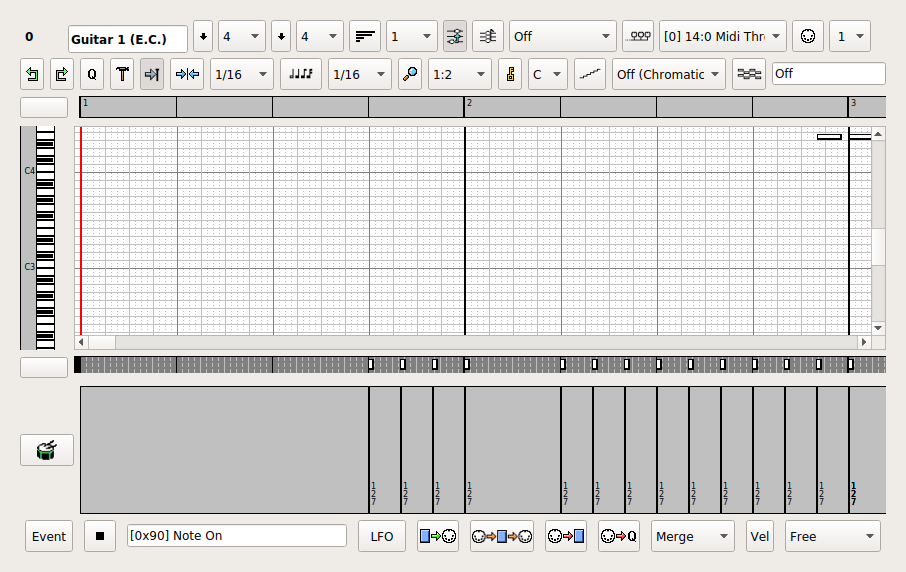
\includegraphics[scale=0.65]{roll.png}
%  \caption{Queued-Replace (Queued-Solo) In Action}
%  \label{fig:queued_replace}
% \end{figure}

   Before pressing the "keep queue" key, patterns 33 ("\textbf{q}")
   and 34 ("\textbf{a}") are
   unmuted, while the desired replace pattern, 32 ("\textbf{1}") is off.
   Then the user presses (and holds) the "replace" key, then clicks the
   "\textbf{1}" key.
   This puts all unmuted patterns, plus the muted
   replace pattern as well, into queue mode, as shown by the grey panels.
   When the progress bar reaches the end of the pattern, pattern 32 will go on,
   and patterns 33 and 34 will go off.
   If the replace-pattern is already on, it is not queued, as
   there's no need to turn it on.

   If, while in queue mode, the replace key is held and
   "\textbf{1}" is pressed again,
   the other patterns will be queued, and will turn on again.  Thus, the
   solo status of the replace pattern can be toggled at will, until queue mode
   is exited by pressing and releasing the normal "queue" key.
   If the replace key is \textsl{not} held down, and another pattern's replace
   hot-key is pressed, that pattern will be queued normally.
   If one wants to change the solo functionality to a different pattern,
   simple hold the replace key and click on a different pattern.  The new
   arrangement of soloing is memorized.
   One can clear the queue mode by pressing the normal queue key.

   There are more keys defined in the \textbf{Keyboard} dialog, and it is
   worth figuring out what they do, if not documented here.
   For a couple of short, but good, video tutorials about using arming,
   queuing, and snapshots, see reference \cite{wootangent1}.

\paragraph{Other Pattern Clicks}
\label{paragraph:patterns_pattern_clicks}

   \index{pattern!left click}
   \index{pattern!mute toggle}
   Left-click on a pattern-filled box will change its state
   \index{pattern!mute}
   \index{pattern!unmute}
   from muted (white background) to playing (black background), whether
   the sequencer is playing or not.

   \index{pattern!left click-drag}
   Left-click-hold-drag on a pattern, drags it to a different
   pattern on the grid.
   The box disappears while dragged, and reappears in the new location when
   dropped.  However, a pattern \textsl{cannot} be dragged if its
   \textbf{Pattern Editor} window is open.

   \index{pattern!right click}
   Right-click on a pattern brings up the appropriate context menus, as
   discussed earlier, depending on whether the pattern box is empty or
   filled.

   \index{pattern!middle click}
   Middle-click on a pattern will bring up the pattern in the \textbf{Editor}
   tab in the main window.

   \index{pattern!shift-left-click}
   \index{shift-left-click live-frame}
   A Shift-Left click on a pattern will open up an external live-frame for the
   set having the same number as the pattern.

   \index{pattern!ctrl-left-click}
   \index{ctrl-left-click new pattern}
   A Ctrl-Left click on a pattern will create a new pattern, just like
   double-click will (if enabled).

   \index{solo!true}
   \index{pattern!alt-left-click}
   \index{patterns panel!inverse muting}
   \index{patterns panel!solo}
   \index{alt-left-click solo}
   There is a truer "Solo" functionality in the Patterns
   Panel and the Song Editor.  To "solo" a pattern, move the mouse cursor
   over the pattern, hold the \texttt{Alt} key, and left-click the pattern.
   This will turn off all the other patterns, so that the selected pattern ins
   the only one playing.
   We still need to work on reversing it exactly, but
   mute-groups can be used for that purpose.
%  Holding the \texttt{Alt} key and clicking the same
%  pattern again will unmute all of the other patterns.

\paragraph{Pattern Recording Modes}
\label{paragraph:patterns_recording_modes}

   \textsl{Seq66} has always had the feature of turning on recording, including
   quantized recording, in the pattern editor.
   With version 0.97.3, it also provides for
   \index{recording!modes}
   recording modes.  With this new feature, the normal loop muting/unmuting
   functionality of the \textbf{Live Grid} can be changed to allow the toggling
   of recording of each pattern.
   This new functionality is enabled by two buttons in the main window grid and
   by two refactored keystroke/MIDI controls ("Record" and "Quan Record").
   The normal mode (mute/unmute) is called \textbf{Loop}.

   \begin{itemize}
      \item \textbf{Loop}.
         This mode is the legacy and long-time standard mode of
         \textsl{Seq24}, \textsl{Sequencer64}, and \textsl{Seq66}.
         When in this mode, a click on a pattern slot, a loop-control
         keystroke, or a loop-control MIDI event, will change the mute/unmute,
         armed/unarmed status of a pattern.
      \item \textbf{Record}.
         A click/key on the pattern turns on recording for that pattern.
      \item \textbf{Copy}.
         Copies the selected pattern into the clipboard.
      \item \textbf{Paste}.
         Pastes the clipboard into the selected pattern.
      \item \textbf{Clear}.
         Removes the events from the selected pattern.  Careful!
         Not yet ready.
      \item \textbf{Delete}.
         Deletes the selected pattern.  Careful!
      \item \textbf{Thru}.
         Turns on the MIDI Thru functionality of the selected pattern.
      \item \textbf{Solo}.
         Soloes the selected pattern.
      \item \textbf{Cut}.
         Deletes the selected pattern and copies it into the clipboard.
      \item \textbf{Double}.
         Doubles the length of the selected pattern.
         Not yet ready.
   \end{itemize}
   It has been supplemented by four recording modes.
   Here are the modes:

   \begin{itemize}
      \item \textbf{Overdub}.
         \index{merge}
         \index{overdub}
         \index{record!merge}
         \index{record!overdub}
         This mode is selected by clicking on the \textbf{Loop} button,
         then using the \textbf{Record} control.
         These commands cycle between all the modes in this list.
         Overdub is the same as the \textbf{Merge} option in the 
         pattern editor.
         Clicking a grid will turn on/off the overdub recording mode
         for that pattern.
         It enables recording that accumulates note events in each pass of
         looping through the pattern.
      \item \textbf{Overwrite.}
         \index{overwrite}
         \index{recording!overwrite}
         This mode causes the grid button to turn on overwrite recording.
         When the loop restarts over and a note is pressed,
         then the existing notes in that loop are erased,
         and the new note is added.
      \item \textbf{Expand}.
         \index{expand}
         \index{recording!expand}
         This mode causes the grid button to turn on expand recording.
         Once the end of the loop is near, whether or
         not any notes are being input, another measure is added to the length
         of the loop.
      \item \textbf{One-shot}.
         \index{one-shot}
         \index{recording!one-shot}
         When this option is set, with the record button on, and no pattern
         playing, recording won't start until a note comes in, and when the
         first note comes in, the progress bar starts at the left (time 0).
         As each new set of notes at the same timestamp come in, the
         notes are recorded and the current time advances by one snap value.
         Once the end of the pattern lenght is reached, recording is turned
         off.
      \item \textbf{One-shot Reset}.
         \index{one-shot reset}
         \index{recording!one-shot reset}
         When the \textbf{One-shot} option is selected, this new option
         is enabled.
         When clicked, three things happen:
         \begin{itemize}
            \item All the (note) events just recorded are \textsl{erased}.
            \item One-short counters/flags are \textsl{reset}.
            \item Recording is turned \textsl{back on}.
         \end{itemize}
         Thus, one can easily re-do a one-short recording.
   \end{itemize}

   Once the recording mode is turned on, then the recording type comes into
   play:

   \begin{itemize}
      \item \textbf{No Quan}.
         Incoming events are recorded as is.
         Plain recording, events recorded with timestamps unaltered.
         Indicated by a red circle.
      \item \textbf{Quantize}.
         When recording, quantize the incoming events.
         Incoming events are quantized to the snap value of the pattern.
         Indicated by a red circle and a "Q" inside it in a pattern slot.
      \item \textbf{Tighten}.
         A weaker version of \textbf{Quantize}.
         Incoming events are partially quantized to the snap value of the
         pattern.
         Indicated by a red circle and a "T" inside it in a pattern slot.
         This mode is accessible only via this recording mode; there
         is no such button in the pattern editor.
   \end{itemize}

\subsection{Patterns / Bottom Panel}
\label{subsec:patterns_panel_bottom}

   The first line of the bottom panel contains the \textbf{Set Name}
   of the current set, which is editable.
   It contains a button with an exclamation point (\textbf{!}), which
   can be used to reset the play-set (the total of all patterns that are loaded
   for playback) to the patterns in the current set.
   The \textbf{Set} spin-box can be used to change the current set.

   \begin{enumber}
      \item \textbf{Set Name}
      \item \textbf{Set Reset}
      \item \textbf{Set}
   \end{enumber}

   \setcounter{ItemCounter}{0}      % Reset the ItemCounter for this list.

   \itempar{Set Name}{pattern!set name}
   Each of the 32 available screen-sets can be given a name by entering it
   into this field.  This name is saved with the MIDI file.

   \itempar{Set}{pattern!set number}
   This spin widget selects the current screen-set.  The values in this
   field range from 0 to 31 (less if the set-size is a larger value),
   and default to 0.

   \itempar{Set Reset}{pattern!set reset}
   \textsl{Seq66} has a new feature whereby multiple sets can play at once.
   This button, an exclamation point, will reset the playback to the patterns
   in the current set.

   The bottom panel of the Patterns window provides way to control the
   overall playback of the song.  It has changed quite a bit over the last few
   versions of \textsl{Seq66}, and we have not yet caught up with the
   diagrams. And the Qt user-interface adds more changes.
   Refer to the diagram of the whole window, for now.
   It has a number of items:

   \begin{enumber}
      \item \textbf{Panic!}
      \item \textbf{Stop}
      \item \textbf{Play and Pause}
      \item \textbf{Loop}
      \item \textbf{Song Record}
%     \item \textbf{Song Record Snap}
%     \item \textbf{Log Tempo}
%     \item \textbf{Record Tempo}
      \item \textbf{Keep-Queue Status}
      \item \textbf{Toggle Song/Live Mode}
      \item \textbf{Tap Tempo}
      \item \textbf{BPM}
   \end{enumber}

   \setcounter{ItemCounter}{0}      % Reset the ItemCounter for this list.

   \itempar{Panic!}{pattern!panic}
   This new button stops the song and sends MIDI Off messages on all notes.

   \itempar{Stop}{pattern!stop}
   The red square button stops the playback of the song and all its patterns.
   \index{keys!esc (stop)}
   The keystroke for stopping playback is the \texttt{Escape} character; it
   stops playback and rewinds to the beginning of the song.
   The \texttt{Space} keystroke will do the same thing if playback is in
   progress; it is effectively a playback toggle key.

   \itempar{Play and Pause}{pattern!Play}
   \index{pattern!Pause}
   The green triangular button starts the playback of the whole song.
   \index{keys!space (play)}
   The keystroke for starting playback is the \texttt{Space} character by
   default.  It also stops playback, also rewinding the song to the beginning.

   \index{pause}
   The Pause button toggles playback without rewinding the song.
   A Pause key (by default, the period) is also defined.

   \itempar{Loop}{pattern!loop}
   If this button is active, then the playback will loop
   between the "L" and "R" markers in the pattern editor or the song editor
   time-lines.

   \itempar{Song Record}{pattern!song record}
   Song-recording in \textsl{Seq66} is adopted from the
   \textsl{Kepler34} project.
   This feature takes live muting changes and records them as
   triggers in the \textbf{Song Editor}.
   The default hot-key for this function is \texttt{P}.
   This feature does not honor queuing...
   rather than waiting until the end of the pattern when the queuing takes
   effect, the trigger recording starts immediately.

%  \itempar{Song Record Snap}{pattern!song record snap}
%  This button toggles snapping the beginning and end of a recorded trigger to
%  the nearest beat.  There is no hot-key for this button at this time.
%  And, in fact, at present, song-record snap is alway in force.

   \itempar{BPM}{pattern!BPM}
   The spin widget adjusts the "beats per minute" (BPM) value.  The
   range of this field is from 1 bpm to 600 bpm, with a default value of
   120 bpm.
   Although this field looks editable, it is not.  Most keystrokes
   that are entered actually toggle one of the pattern boxes.
   However, the following keys can also modify the BPM in small increments:
   \index{keys!semicolon}
   The \texttt{semicolon} reduces the BPM;
   \index{keys!apostrophe}
   The \texttt{apostrophe} increases the BPM.
   Also, if one right-clicks on the Up button, the BPM advances to its largest
   supported value, and if one right-clicks on the Down button, the BPM
   advances to its lowest value.
   MIDI control for this value is also available.

   The precision of the BPM value can be set to 0, 1, or 2
   decimal places, and the increment values for the step size (small)
   or page size (large) of the BPM spinner can be configured in the 'usr' file.

   \itempar{Tap Tempo}{pattern!tap tempo}
   This control is clicked in time with a tune, to set the
   tempo based on the tempo of the clicks.  Once clicked, the label of this
   button increments with every click, and the \textbf{BPM} field updates to
   display the calculated tempo.  If the user stops tapping for 5 seconds, the
   label reverts to 0, the BPM value keeps its final value, and the user can
   try tapping the tempo again, or accept the current value.
   Tapping can also be done using the keystroke defined
   in the 'ctrl' file.
   It defaults to the "\texttt{F9}" key.

   \itempar{Keep-Queue Status}{pattern!keep-queue}
   This item is the \textbf{Q} button.
   It provides a visual way to know the current state of keep-queue, and is
   activated either by clicking on it or by pressing the assigned keep-queue
   key.

   \itempar{Toggle Song/Live Mode}{pattern!song/live}
   Pressing this button toggles between the song mode and live mode.
   Note that the default mode is configurable, and \textsl{Seq66} can go into
   song mode when a loaded MIDI file has triggers, if configured to do so.

\subsection{Patterns / Multiple Panels}
\label{subsec:patterns_panel_multiple}

   Multiple patterns-panels can be created in addition to the one in the "Live"
   tab.  The live set-up and set-down keystrokes, as well as their MIDI control
   counterparts (both defined in a 'ctrl' file).
   apply only to the main window.

%  Of course, if the "mainwnds" are synced, then all are affected by these
%  keystrokes.
%
%  In multi-wid mode, each "mainwnd" frame shows the corresponding set number
%  and, if present, the set name text for each "mainwnd" set.
%
%  The \texttt{-o wid=3x2,i} option can be used to set this mode.
%  These settings can be made permanent in the 'usr' file.
%  In that file, the options modified are \texttt{block\_rows} and
%  \texttt{block\_columns}.

\subsection{Patterns / Variable Set Size}
\label{subsec:patterns_panel_variset}

   \index{variset}
   This option, informally known as "variset", allow some changes in
   the set size and layout from the default 4x8 = 32 sets layout.
   The row count can be set from 4 to 8, and the column count can be set to 8
   to 12.  Note that the set size can only be \textsl{increased} by these
   settings.

   \textbf{Warning:}
   \textsl{seq24} was fairly hardwired for supporting 32 patterns per
   set, and there are still places where that is true.  Thus,
   consider this option to be experimental.

   The \texttt{-o sets=8x8} option can be used to set this mode.
   These settings can be made permanent in the 'usr' file.
   In that file, the options modified are \texttt{mainwnd\_rows} and
   \texttt{mainwnd\_cols}.

   Generally, it is recommend to stick with the 4x8 (32 patterns/set),
   8x8 (64 patterns/set), and 8x12 (96 patterns/set).  This works best with the
   existing set of 32 hot-keys.

   Also note that the Qt 5 user-interface also supports "variset", whether in
   the main window or in the external live-frame.  In addition, the Qt windows
   can be resized and still show reasonable renditions of the pattern-slots.

\subsection{Patterns / Set Handling}
\label{subsec:patterns_panel_set_handling}

   Let's go through an example using the \texttt{Home} key (or whatever key is
   configured as the \textbf{Set Playing Screenset} key.)

   \begin{enumber}
      \item Load a song with more than one screen-set.
      \item Unmute the pattern(s) in the first set and start playback.
      \item Use the "\texttt{]}" (\textbf{Screenset Up}) key to move to the next
         set.  Note that the first set is still playing.  Also note that the
         now-current set is \textsl{not} playing.
      \item Press the \texttt{Home} key.
         Note that the first set turns off, and the current set turns on.
         These steps can be repeated at will.
      \item Finally, hit the \texttt{F8} (\textbf{Toggle Mutes}) key.
         Note that all tracks on all sets toggle muting each time this key is
         pressed.
   \end{enumber}

%-------------------------------------------------------------------------------
% vim: ts=3 sw=3 et ft=tex
%-------------------------------------------------------------------------------
